\section{Atividade 3 -- OSINT com Maltego}

\paragraph{}
Nesta atividade foi utilizada a ferramenta Maltego Community Edition (CE) para
realizar uma análise de OSINT utilizando a transformação \textit{Have I Been
Pwned?}, com o objetivo de identificar possíveis vazamentos de dados associados
a um endereço de e-mail.

\subsection{Procedimento Realizado}

Inicialmente foi criada uma nova análise (\textit{New Graph}) no Maltego e
adicionada uma entidade do tipo \textit{Email Address}. Em seguida, foi
informado o endereço de e-mail definido para a atividade e executada a
transformação disponibilizada pelo plugin \textit{Have I Been Pwned?},
instalado previamente através do \textit{Transform Hub}.

\begin{figure}[H]
\centering
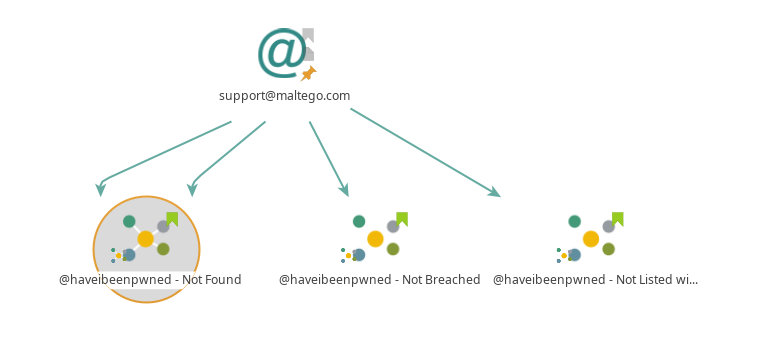
\includegraphics[width=0.95\textwidth]{./fig/atividade3-maltego.png}
\caption{Resultado da transformação utilizando o plugin Have I Been Pwned? no
Maltego.}
\end{figure}

\subsection{Análise dos Resultados}

\paragraph{}
Após a execução da transformação, o Maltego realizou consultas em bases de
dados públicas de vazamentos e apresentou os resultados em formato gráfico,
permitindo visualizar os relacionamentos entre o endereço de e-mail analisado e
os incidentes de segurança identificados.

\paragraph{}
Os nós gerados pela ferramenta exibem informações relevantes sobre cada
vazamento encontrado, incluindo o nome do serviço afetado, a origem do
incidente e outros metadados disponibilizados pela plataforma consultada.

\paragraph{}
A representação gráfica fornecida pelo Maltego facilita a correlação das
informações coletadas, permitindo compreender rapidamente a exposição do
endereço analisado e identificar possíveis riscos decorrentes da reutilização
de credenciais ou do comprometimento de dados pessoais.

\paragraph{}
A atividade demonstrou a utilidade das ferramentas de OSINT para obtenção e
correlação de informações disponíveis em fontes abertas, evidenciando como
dados expostos em vazamentos podem ser utilizados durante atividades de
reconhecimento e análise de segurança.
